\documentclass[a4paper, 12pt]{article}

\newcommand{\languages}{english, french}

%%%%% Tools

\usepackage{comment}
\usepackage{lipsum}
\usepackage{xstring}

%%%%% Document

\usepackage{hyperref}
\usepackage{geometry}
\usepackage{fancyhdr}
\usepackage[parfill]{parskip}

\geometry{paper=a4paper,top=3.5cm,bottom=2.5cm,right=2.5cm,left=2.5cm}

\pagestyle{fancy}
\fancyhead[L]{}
\fancyhead[R]{\leftmark}
\fancyfoot[C]{\thepage}
\renewcommand{\headrulewidth}{0pt}

%%%%% Text

\usepackage[utf8]{inputenc}
\usepackage[T1]{fontenc}

\newlength{\mytextsize}
\makeatletter
\setlength{\mytextsize}{\f@size pt}
\makeatother

%%%%% Languages

\usepackage[\languages]{babel}

% english

\addto\captionsenglish{\def\figurename{Figure}}
\addto\captionsenglish{\def\tablename{Table}}

\newcommand{\st}{\text{s.t.}}

\IfStrEq{\languagename}{english}{
	\newcommand{\lgpreamble}{Preamble}
}

% french

\frenchbsetup{StandardLists=true}

\addto\captionsfrench{\def\figurename{Figure}}
\addto\captionsfrench{\def\tablename{Tableau}}
\addto\captionsfrench{\def\proofname{Preuve}}

\newcommand{\tq}{\text{t.q.}}
\newcommand{\cad}{c.-à-d. }
\newcommand{\Cad}{C.-à-d. }

\IfStrEq{\languagename}{french}{
	\newcommand{\lgpreamble}{Préambule}
}

%%%%% Styles

\usepackage[skip=\mytextsize]{caption}
\usepackage{float}
\usepackage{mdframed}
\usepackage{enumitem}
\usepackage{eurosym}
\usepackage{color}

\newcommand\caaption[1]{\caption{#1}\vspace{-1.5\mytextsize}}

%%%%% Mathematics

\usepackage{amsmath}
\usepackage{amssymb}
\usepackage{amsfonts}
\usepackage{bm}
\usepackage{esint}
\usepackage[makeroom]{cancel}

\newcommand{\fact}[1]{#1!}
\newcommand{\deriv}{\mathrm{d}}
\DeclareMathOperator{\tr}{tr}

%%%%% SI units

\usepackage[squaren,Gray,cdot]{SIunits}
\usepackage{sistyle}

\IfStrEq{\languagename}{french}{
	\SIdecimalsign{,}
}

%%%%% Chemistry

\usepackage[version=4]{mhchem}

%%%%% Table & Figure

\usepackage{array}
\usepackage{tabularx}
\usepackage{multirow}
\usepackage{multicol}
\newcolumntype{M}[1]{>{\centering\arraybackslash}m{#1}}
%\setlength\extrarowheight{0em}
\renewcommand{\arraystretch}{1.3}

\usepackage{pgfplots}
\usepackage{tikz}
\usetikzlibrary{shapes.geometric, positioning}
\usepackage{graphics}
\usepackage{graphicx}
\pgfplotsset{axis on top, compat = 1.3}

%%%%%% Theorems and Definitions

\usepackage{amsthm}
\usepackage{thmtools}

\IfStrEq{\languagename}{english}{
	\newcommand{\lgthm}{Theorem}
	\newcommand{\lglem}{Lemma}
	\newcommand{\lgprop}{Proposition}
	\newcommand{\lgdefn}{Definition}
	\newcommand{\lghyp}{Hypothesis}
	\newcommand{\lgquest}{Question}
	\newcommand{\lgansw}{Answer}
	\newcommand{\lgexpl}{Example}
	\newcommand{\lgrmk}{Remark}
	\newcommand{\lgnote}{Note}
	\newcommand{\lgtip}{Tip}
}

\IfStrEq{\languagename}{french}{
	\newcommand{\lgthm}{Théorème}
	\newcommand{\lglem}{Lemme}
	\newcommand{\lgprop}{Proposition}
	\newcommand{\lgdefn}{Définition}
	\newcommand{\lghyp}{Hypothèse}
	\newcommand{\lgquest}{Question}
	\newcommand{\lgansw}{Réponse}
	\newcommand{\lgexpl}{Exemple}
	\newcommand{\lgrmk}{Remarque}
	\newcommand{\lgnote}{Note}
	\newcommand{\lgtip}{Conseil}
}

\theoremstyle{plain}
\newtheorem{thm}{\lgthm}[section]
\newtheorem{lem}{\lglem}[section]
\newtheorem{prop}{\lgprop}[section]

\theoremstyle{definition}
\newtheorem{defn}{\lgdefn}[section]
\newtheorem{hyp}{\lghyp}[section]
\newtheorem{quest}{\lgquest}[]

\declaretheorem[
name=\lgansw,
qed={\lower-0.3ex\hbox{$\triangle$}},
within=quest
]{answ}

\declaretheorem[
name=\lgexpl,
qed={\lower-0.3ex\hbox{$\triangle$}},
within=section
]{expl}

\theoremstyle{remark}
\newtheorem*{rmk}{\lgrmk}
\newtheorem*{note}{\lgnote}
\newtheorem*{tip}{\lgtip}

\begingroup
\makeatletter
\@for\theoremstyle:=definition,remark,plain\do{%
	\expandafter\g@addto@macro\csname th@\theoremstyle\endcsname{%
		\addtolength\thm@preskip\parskip
	}%
}
\endgroup

%%%% Others

\renewcommand{\qedsymbol}{$\blacksquare$}

%%%%%%%%%%%%%%%%%%%

%%%%%%%%%%%%%%%%%%%

\title{Projet 1 - Jeu de Hasard}
\newcommand{\subtitle}{Éléments du Calcul des Probabilités}
\author{François \textsc{Rozet} (s161024)\\Jules \textsc{Remes} (s162964)\\}
\newcommand{\context}{2\up{ème} année de Bachelier Ingénieur civil}
\date{Année académique 2017 - 2018}

%%%%%%%%%%%%%%%%%%%

\usepackage{colortbl}
\usepackage{listings}

\def\lstbasicfont{\fontfamily{pcr}\selectfont}

\lstdefinestyle{MatLab}{
	language=Matlab,
	%%%%%%
	showstringspaces=false,
	extendedchars=true,
	tabsize=4,
	columns=fixed,
	%%%%%%
	breaklines=true,
	breakatwhitespace=true,
	prebreak=\space,
	%%%%%%
	basicstyle=\fontfamily{pcr}\footnotesize,
	keywordstyle=\color{blue!60!black},
	commentstyle=\itshape\color{green!40!black},
	stringstyle=\color[rgb]{.627,.126,.941},
	%%%%%%
	morekeywords={ones, parfor, var, randi, normrnd, table, clearvars, getGain, getProb, doSim, getLength},
	%%%%%%
	numbersep=0.5\mytextsize,
	numbers=left,
	numberstyle={\lstbasicfont\footnotesize},
	%%%%%%
	frame=single,
	rulecolor=\color{black},
	framexleftmargin=2\mytextsize,
	xleftmargin=2\mytextsize,
	captionpos=b,
	aboveskip=1\mytextsize,
	belowskip=1\mytextsize
}

\renewcommand{\thesubsection}{(\alph{subsection})}

%%%%%%%%%%%%%%%%%%%

\begin{document}
	\newgeometry{margin = 2.5cm}
\makeatletter
\begin{titlepage}
	\begin{minipage}[t][0.425\textheight][t]{\textwidth}
		\begin{center}
			
\includegraphics[height=0.15\textheight]{include/resources/pdf/logo_uliege.pdf}
			\vfill
			{\huge \textsc{Université de Liège}}
			\vfill
		\end{center}
	\end{minipage}
	\vfill
	\begin{minipage}{\textwidth}
		\hspace{6pt}
		\begin{mdframed}[linewidth = 2pt, innertopmargin = 12pt, innerbottommargin = 12pt, leftline = false, rightline = false]
			\begin{center}
				{\huge \bfseries \@title}
			\end{center}
		\end{mdframed}
		\hspace{6pt}
	\end{minipage}
	\vfill
	\begin{minipage}[b][0.425\textheight][t]{\textwidth}
		\begin{center}
			\ifx\subtitle\undefined
			\else
			{\LARGE \subtitle}
			\fi
			\vfill
			{\large \@author}
			\vfill
			{\large \context \\[6pt] \@date}
		\end{center}
	\end{minipage}
\end{titlepage}
\makeatother
\restoregeometry
	\newpage
	\section{Lehman \& Leighton}
	\subsection{Position initiale aléatoire}
	Si le joueur choisit aléatoirement la position initiale de la balle, on peut supposer que ses quatre choix possibles sont équiprobables. On suppose aussi que, à chaque bifurcation, la direction prise par la bille est choisie aléatoirement et de façon équiprobable.
	\begin{figure}[H]
		\centering
		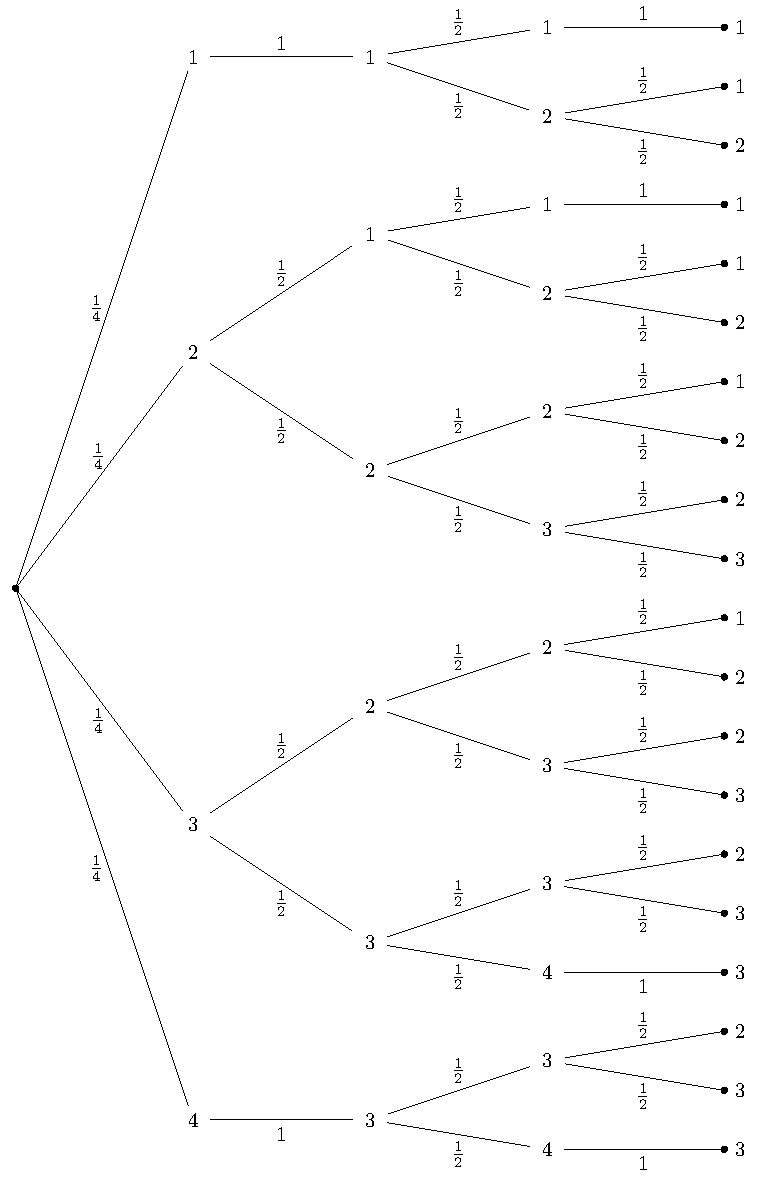
\includegraphics[scale = 0.95]{resources/tikz/lehman_leighton_full/lehman_leighton_full.pdf}
		\caaption{Arbre de probabilité pour un départ aléatoire.}
		\label{figure: Q1a}
	\end{figure}
	En considérant les collections d'évènements $\varepsilon_1$, $\varepsilon_2$ et $\varepsilon_3$ qui rassemblent, respectivement, les chemins donnant lieux aux sorties $1$, $2$ et $3$, on obtient les probabilités d'occurrence données dans le tableau \ref{table: Q1a}.
	\begin{table}[H]
		\centering
		\begin{tabular}{|c|c|c|}
			\hline
			$P(A \in \varepsilon_1)$ & $P(A \in \varepsilon_2)$ & $P(A \in \varepsilon_3)$ \\ \hline\hline
			\multirow{2}{*}{$\dfrac{11}{32}$} & \multirow{2}{*}{$\dfrac{10}{32}$} & \multirow{2}{*}{$\dfrac{11}{32}$} \\
			&& \\ \hline	
			$\num{0.34375}$ & $\num{0.3125}$ & $\num{0.34375}$ \\ \hline
		\end{tabular}
		\caption{Distribution de probabilité théorique pour un départ aléatoire.}
		\label{table: Q1a}
	\end{table}
	\subsection{Position initiale fixée}
	Lorsque le joueur choisit toujours la position initiale la plus à gauche, \cad $1$, l'arbre se réduit à une seule de ses branches principales.
	\begin{figure}[H]
		\centering
		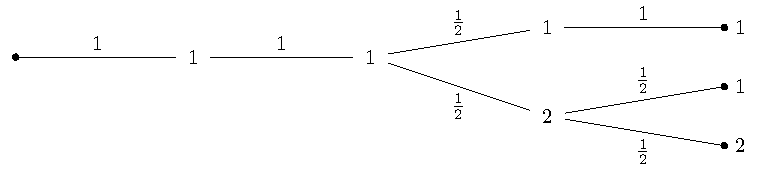
\includegraphics[scale = 0.95]{resources/tikz/lehman_leighton_1/lehman_leighton_1.pdf}
		\caaption{Arbre de probabilité pour le départ $1$.}
	\end{figure}
	Et, pour les mêmes collections que précédemment, on trouve les résultats contenus dans le tableau \ref{table Q1b}.
	\begin{table}[H]
		\centering
		\begin{tabular}{|c|c|c|}
			\hline
			$P(A \in \varepsilon_1)$ & $P(A \in \varepsilon_2)$ & $P(A \in \varepsilon_3)$ \\ \hline\hline
			\multirow{2}{*}{$\dfrac{3}{4}$} & \multirow{2}{*}{$\dfrac{1}{4}$} & \multirow{2}{*}{$0$} \\
			&& \\ \hline	
			$\num{0.75}$ & $\num{0.25}$ & $\num{0}$ \\ \hline
		\end{tabular}
		\caaption{Distribution de probabilité théorique pour le départ $1$.}
		\label{table: Q1b}
	\end{table}
	On peut remarquer que, dans les deux cas étudiés, la somme des probabilités d'occurrence associées aux trois collections d'évènements vaut $1$, vérifiant ainsi le second axiome de Kolmogorov.
	\newpage
	\section{Monte Carlo}
	\subsection{Simulation simplifiée et estimation de probabilité}
	Dans le script \texttt{Q2a.m}\footnote{Les scripts, et les fonctions qu'ils utilisent, sont disponibles dans l'annexe.}, on génère, en premier lieu, un vecteur d'entrées \texttt{in}. Dans le cas où la position initiale est aléatoire, il est créé à partir de la fonction \texttt{randi} et dans l'autre cas, ses éléments sont fixés à $1$ par la fonction \texttt{ones}. \par
	Ensuite, la fonction \texttt{doSim}, prenant en argument le vecteur \texttt{in} et les paramètres du problème, simule une sortie pour chacune des entrées. Ce vecteur de sorties permet à la fonction \texttt{getProb} de calculer les fréquences d'occurrences relatives de ces dernières et donc de construire l'estimateur de la distribution de probabilité demandée. \par
	Les résultats obtenus, renseigné dans tableau \ref{table: Q2a1}, en exécutant le script sont relativement proches des valeurs théoriques.
	\begin{table}[H]
		\centering
		\begin{tabular}{|c|c|c|c|}
			\hline
			\textbf{Taille} $= \num{e4}$ & $P(A \in \varepsilon_1)$ & $P(A \in \varepsilon_2)$ & $P(A \in \varepsilon_3)$ \\ \hline\hline
			            (a)              &      $\num{0.3394}$      &      $\num{0.3191}$      &      $\num{0.3415}$      \\ \hline
			            (b)              &      $\num{0.7559}$      &      $\num{0.2441}$      &        $\num{0}$         \\ \hline
		\end{tabular}
		\caaption{Estimations de distributions de probabilité.}
		\label{table: Q2a1}
	\end{table}
	Suite à plusieurs essais, on note qu'augmenter la taille du vecteur d'entrées permet d'améliorer la précision de la méthode.
	\begin{table}[H]
		\centering
		\begin{tabular}{|c|c|c|c|}
			\hline
			\textbf{Taille} $= \num{e5}$ & $P(A \in \varepsilon_1)$ & $P(A \in \varepsilon_2)$ & $P(A \in \varepsilon_3)$ \\ \hline\hline
			            (a)              &      $\num{0.3440}$      &      $\num{0.3143}$      &      $\num{0.3417}$      \\ \hline
			            (b)              &      $\num{0.7491}$      &      $\num{0.2509}$      &        $\num{0}$         \\ \hline
		\end{tabular}
		\caption{Estimations de distributions de probabilité.}
		\label{table: Q2a2}
	\end{table}
	\subsection{Simulation complète et estimation de l'espérance}
	Ici, et pour chaque taille du vecteur d'entrées, les sorties générées par la fonction \texttt{doSim} sont utilisées par la fonction \texttt{getGain} pour déterminer le gain qu'elles génèrent séparément. \par
	Ensuite, la fonction \texttt{mean} calcule la moyenne de ces gains pour l'utiliser en tant qu'estimateur de l'espérance. \par
	Après avoir lancé le script \texttt{Q2b.m} à trois reprises, on observe des variations significatives dans les résultats qu'il retourne et qui sont fournis dans la table \ref{table: Q2b}.
	\begin{table}[H]
		\centering
		\begin{tabular}{|c|c|c|c|c|c|}
			\hline
			         &                       \textbf{Taille}                        &   $\num{e1}$   &  $\num{e2}$   &  $\num{e3}$   &  $\num{e4}$   \\ \hline\hline
			Test $1$ & \multirow{3}{*}{\textbf{Espérance} $\big[\text{\euro}\big]$} & $\num{1.200}$  & $\num{0.280}$ & $\num{0.506}$ & $\num{0.522}$ \\ \cline{1-1}\cline{3-6}
			Test $2$ &                                                              & $\num{-2.100}$ & $\num{0.870}$ & $\num{0.432}$ & $\num{0.540}$ \\ \cline{1-1}\cline{3-6}
			Test $3$ &                                                              & $\num{1.600}$  & $\num{0.400}$ & $\num{0.330}$ & $\num{0.402}$ \\ \hline
		\end{tabular}
		\caaption{Estimations de l'espérance en variant la taille de l'échantillon.}
		\label{table: Q2b}
	\end{table}
	Bien que les valeurs semblent converger vers un nombre avoisinant $\num{0.5}$ lorsque la taille du vecteur augmente, les variations qu'elles subissent restent trop grande pour qu'elles soient représentatives.
	\subsection{Étude de la variance de l'espérance}
	Il s'agit, pour cette question, de répéter l'expérience précédente \texttt{nbrRepeat} (\cad $\num{e3}$) fois. Ensuite, pour chaque taille du vecteur de sorties, les moyenne et variance des \texttt{nbrRepeat} estimations de l'espérance sont déterminées respectivement grâce aux fonctions \texttt{mean} et \texttt{var}.
	\begin{table}[H]
		\centering
		\begin{tabular}{|c|c|c|c|c|c|}
			\hline
			              \textbf{Taille}                &  $\num{e1}$   &    $\num{e2}$    &    $\num{e3}$    &    $\num{e4}$    &    $\num{e5}$    \\ \hline\hline
			 \textbf{Moyenne} $\big[\text{\euro}\big]$   & $\num{0.436}$ &  $\num{0.465}$   &  $\num{0.479}$   &  $\num{0.470}$   &  $\num{0.472}$   \\ \hline
			\textbf{Variance} $\big[\text{\euro}^2\big]$ & $\num{2.656}$ & $\num{2.907e-1}$ & $\num{2.666e-2}$ & $\num{2.703e-3}$ & $\num{2.699e-4}$ \\ \hline
		\end{tabular}
		\caaption{Étude des estimations de l'espérance.}
		\label{table: Q2c}
	\end{table}
	On observe à partir des valeurs calculées par le script \texttt{Q2c.m}, présentées dans le tableau \ref{table: Q2c}, que les moyennes respectives des espérances estimées sont plutôt proches les unes des autres. Au contraire, la variance semble diminuer de la même façon que la taille du vecteur augmente. \par 
	Cependant, pour la taille $\num{e4}$, si on approxime l'erreur moyenne par l'écart type, \cad par la racine de la variance, on trouve qu'elle est de l'ordre d'un dixième de l'espérance, ce qui n'est pas négligeable.
	\begin{align*}
	    \delta \simeq \sigma = \sqrt{\num{2.703e-3}} = \num{5.200e-2}
	\end{align*}
	Dès lors, il est parfaitement envisageable de choisir une taille de $\num{e5}$, voir même plus, si on souhaite augmenter notre précision et que le temps de calcul ne nous rebute pas. \par
	On peut calculer facilement que l'erreur moyenne subira une diminution d'un facteur $\sqrt{10}$ lorsque on multipliera la taille par $10$.
	\subsection{Détermination de la position initiale d'espérance maximale}
	Cette expérience réutilise le code écrit pour la question 2b aux exceptions près que les entrées ne sont plus aléatoires et que le changement du nombre de simulations est remplacé par le changement de la position fixée. \par
	Les résultats du script \texttt{Q2d.m}, donné dans le tableau \ref{table: Q2d}, indiquent que la position initiale dont on peut espérer le gain le plus élevé est la $6$\up{ème}.
	\begin{table}[H]
		\centering
		\begin{tabular}{|c|c|c|c|c|c|>{\columncolor[gray]{0.9}}c|c|c|c|}
			\hline
			             \textbf{Position}              &      $1$       &      $2$      &      $3$      &      $4$      &      $5$      &      $6$      &      $7$      &      $8$      &      $9$      \\ \hline\hline
			\textbf{Espérance} $\big[\text{\euro}\big]$ & $\num{-0.109}$ & $\num{0.022}$ & $\num{0.318}$ & $\num{0.572}$ & $\num{0.707}$ & $\num{0.755}$ & $\num{0.731}$ & $\num{0.647}$ & $\num{0.601}$ \\ \hline
		\end{tabular}
		\caption{Estimations de l'espérance en variant la position initiale.}
		\label{table: Q2d}
	\end{table}
	\subsection{Expériences de Bernoulli et loi binomiale}
		Chaque déviation de la bille peut être considérée comme une expérience de Bernoulli. Ainsi, suivre son chemin le long de la planche revient à étudier la répétition de $9$ expériences de Bernoulli. \par
		Si la réussite de ces dernières est associée à l'évènement \og{}déviée à droite\fg{} dont la probabilité d'occurrence est $\frac{1}{2}$, la loi suivie par la variable aléatoire $\mathcal{X}$ est définie par la loi binomiale $\mathcal{B}\left(9,\frac{1}{2}\right)$. \par
		Dès lors, l'espérance et la variance de $\mathcal{X}$ sont facilement déterminables :
		\begin{align*}
			E\left\{\mathcal{X}\right\} & = 9 \frac{1}{2} = \frac{9}{2} & V\left\{\mathcal{X}\right\} & = 9 \frac{1}{2} \left(1 - \frac{1}{2}\right) = \frac{9}{4}
		\end{align*}
		\subsection{Théorème de Moivre-Laplace et loi de Cauchy}
		\subsubsection*{Théorème de Moivre-Laplace}
		En toute généralité, si $\mathcal{X}_n$ est définie par la loi binomiale $\mathcal{B}\left(n,p\right)$, on sait que :
		\begin{align*}
		E\left\{\mathcal{X}_n\right\} & = np = \mu & V\left\{\mathcal{X}_n\right\} & = n p \left(1 - p\right) = \sigma^2
		\end{align*}
		Or, d'après le théorème de Moivre-Laplace,
		\begin{alignat*}{2}
		&& \left(\frac{\mathcal{X}_n - np}{\sqrt{n p \left(1 - p\right)}}\right) & \xrightarrow{\mathcal{L}} \mathcal{N}(0,1) \\
		\Rightarrow \quad && \mathcal{X}_n & \xrightarrow{\mathcal{L}} \mathcal{N}\left(np,n p \left(1 - p\right)\right)
		\end{alignat*}
		On peut donc approximer la loi binomiale $\mathcal{B}\left(n,p\right)$ par la loi gaussienne (normale) $\mathcal{N}\left(\mu,\sigma^2\right)$ lorsque $n$ augmente. La variable $\mathcal{Y}$ est, quant à elle, approchable par la loi normale $\mathcal{N}\left(0,\sigma^2\right)$. \par
		En pratique, cette approximation est généralement considérée comme acceptable lorsque la variance de $\mathcal{X}_n$ est supérieure ou égale à $10$.
		\begin{align*}
			V\left\{\mathcal{X}_n\right\} = n p \left(1 - p\right) \geq 10
		\end{align*}
		Dans notre cas, $p$ valant $\frac{1}{2}$, la condition est remplie lorsque $n$ est supérieur ou égal à $40$.
		\subsubsection*{Loi de Cauchy}
		Le principe de cette question est le même que celui de la question 2c et, dès lors, leur implémentations est très semblable. On commence par simuler $\num{ek}$ fois la variable $\mathcal{Z}$ comme le rapport de deux instances de la fonction \texttt{normrnd} \cad le rapport de deux variables aléatoires indépendantes suivant une loi normale. \par
		Ensuite, on détermine l'estimateur de l'espérance en calculant la moyenne de ses $\num{ek}$ simulations et on recommence tout ceci $\num{e3}$ fois. \`{A} partir de ces valeurs, on détermine la moyenne et la variance de l'espérance estimée. \par
		Cette méthode, implémentée dans le script \texttt{Q2f.m} pour différentes valeurs de $k$, donne les résultats du tableau \ref{table Q2f}.
		\begin{table}[H]
			\centering
			\begin{tabular}{|c|c|c|c|c|}
				\hline
				              \textbf{Taille}                &   $\num{e2}$    &   $\num{e3}$    &   $\num{e4}$    &   $\num{e5}$    \\ \hline\hline
				 \textbf{Moyenne} $\big[\text{\euro}\big]$   &  $\num{1.281}$  & $\num{-0.7325}$ & $\num{-0.0202}$ & $\num{-2.2852}$ \\ \hline
				\textbf{Variance} $\big[\text{\euro}^2\big]$ & $\num{1.020e4}$ & $\num{4.740e2}$ & $\num{1.403e2}$ & $\num{7.117e3}$ \\ \hline
			\end{tabular}
			\caaption{Étude des estimations de l'espérance de $\mathcal{Z}$.}
			\label{table Q2f}
		\end{table}
		On remarque que l'espérance et la variance de $\mathcal{Z}$ ne convergent pas lorsque la taille des vecteurs de sorties augmente. \par
		L'explication de ce phénomène se trouve dans le fait que la variable aléatoire $\mathcal{Z}$ est définie comme le rapport de deux variables aléatoires indépendantes $\mathcal{Y}_1$ et $\mathcal{Y}_2$ suivant des lois gaussiennes $\mathcal{N}\left(0,2\right)$.
		\begin{align*}
			\mathcal{Z} & = \frac{\mathcal{Y}_1}{\mathcal{Y}_2} \\
			& = \frac{\mathcal{Y}_1}{\sqrt{2}}\frac{\sqrt{2}}{\mathcal{Y}_2}
		\end{align*}
		Cependant, $\frac{\mathcal{Y}_1}{\sqrt{2}}$ suit, ainsi que $\frac{\mathcal{Y}_2}{\sqrt{2}}$, une loi normale $\mathcal{N}\left(0,1\right)$. 
		Dès lors, $\mathcal{Z}$ peut être définie par le rapport de deux lois gaussiennes centrées-réduites, \cad par une loi de Cauchy qui n'admet pas d'espérance et, à fortiori, de variance.
	\newpage
	\appendix
	\section{Scripts}
	\lstinputlisting[style=Matlab, caption={\texttt{Q2a.m}}]{resources/matlab/Q2a.m}
	\lstinputlisting[style=Matlab, caption={\texttt{Q2b.m}}]{resources/matlab/Q2b.m}
	\lstinputlisting[style=Matlab, caption={\texttt{Q2c.m}}]{resources/matlab/Q2c.m}
	\lstinputlisting[style=Matlab, caption={\texttt{Q2d.m}}]{resources/matlab/Q2d.m}
	\lstinputlisting[style=Matlab, caption={\texttt{Q2f.m}}]{resources/matlab/Q2f.m}
	\newpage
	\section{Fonctions}
	Lors de l'écriture des fonctions, nous avons fait le choix de ne pas les rendre robustes, \cad que nous supposons leurs entrées valides et ne les vérifions pas. Ce choix permet de garder les scripts rapides malgré les nombreuses simulations effectuées.
	\lstinputlisting[style=Matlab, caption={\texttt{doSim.m}}]{resources/matlab/doSim.m}
	\lstinputlisting[style=Matlab, caption={\texttt{getProb.m}}]{resources/matlab/getProb.m}
	\lstinputlisting[style=Matlab, caption={\texttt{getGain.m}}]{resources/matlab/getGain.m}
\end{document}